\documentclass{standalone}
\usepackage[utf8]{inputenc}
\usepackage{tikz}
\begin{document}
\usepgflibrary {shadings}
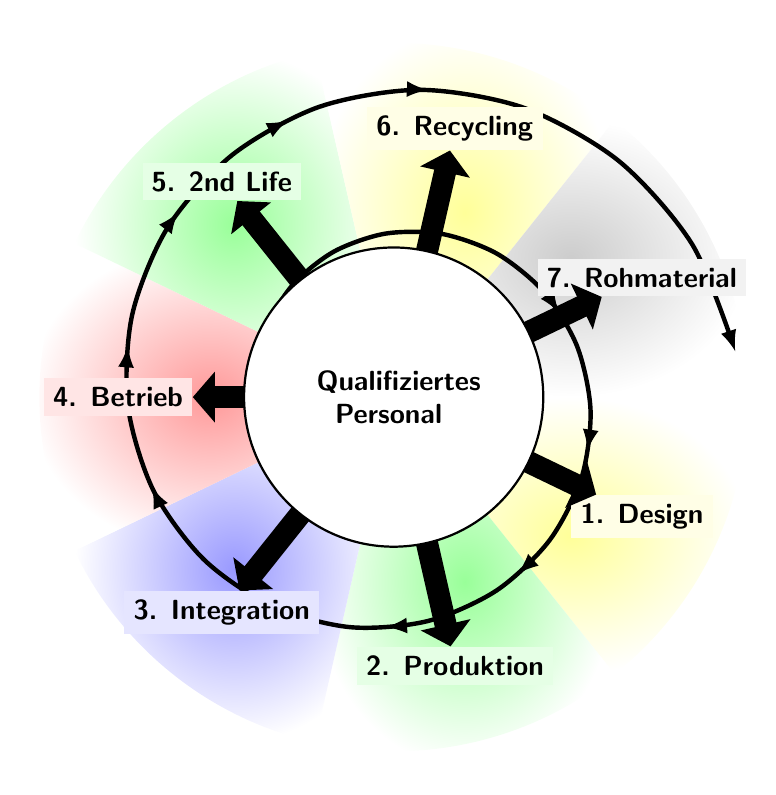
\begin{tikzpicture}[every node/.style={font=\sffamily}]
\def\mycircle{4.5}
\usetikzlibrary{decorations.markings}
\usetikzlibrary{arrows.meta}
\def\phi{51.4285};
\foreach [count=\i] \farb in {yellow, green, blue, red, green, yellow, gray}
\shadedraw[inner color=\farb!40,draw=none] (0:0) -- (-\i*\phi:\mycircle) arc (-\i*\phi:-\i*\phi+\phi:\mycircle) -- cycle;

\begin{scope}[very thick,decoration={
markings,
mark=between positions 0.1 and 0.9 step 0.05 with {\arrow{>}}}
]

\draw[->,>=latex,ultra thick,postaction={decorate}] [domain=0:25,variable=\t,smooth,samples=75]
plot ({-\t r}: {0.007*\t*\t});

\end{scope}

\foreach [count=\i] \farb/\m/\n in {%
yellow/Design/,
green/Produktion/,
blue/Integration/,
red/Betrieb/,
green/2nd Life/,
yellow/Recycling/,
gray/Rohmaterial/%
}
{%
\node[fill=\farb!10] (node\i) at (-\i*\phi+\phi/2:3.5) {\textbf{\i. \m}
};
% \node[fill=white,draw] (mile\n) at (-\i*\phi:5) {\n};
% \draw (mile\n) -- (0:0);
\draw[-{Triangle[width=18pt,length=8pt]}, line width=8pt] (0:0) -- (node\i);
}
\filldraw[fill=white, draw, thick] (0:0) node {\parbox{3cm}{\centering \textbf{
Qualifiziertes\\
Personal
}
}} circle (1.9);
\end{tikzpicture}
\end{document}